\section{gr-isdbt-Tx Un transmisor ISDB-T implementado en SDR}

%\subsection{Comienza seccion 4}
\begin{frame}{gr-isdbt-tx}
\begin{figure}
	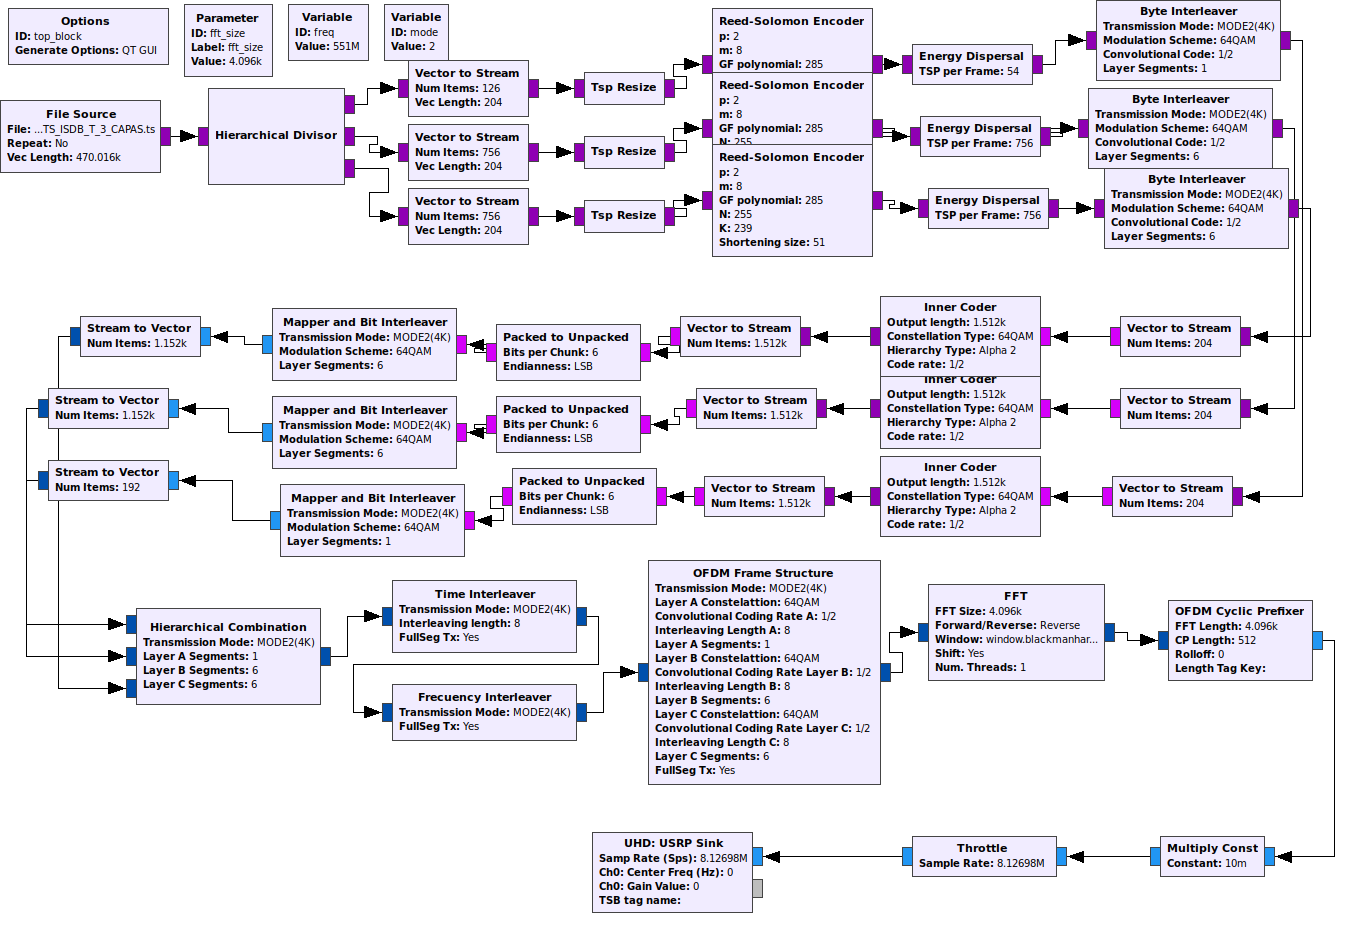
\includegraphics[scale=0.20]{flowgraphEdited}
	\caption{Esquema de bloques de gr-isdbt-Tx en GNU Radio}
\end{figure}
\end{frame}

%\subsection{La entrada de datos}
\begin{frame}
\frametitle{El divisor jerárquico}
	\begin{itemize}	
		\item { Separa TS válidos por capa}
		\item {	Descarta TSP nulos }
		\item { Cada TS continúa a procesamiento individual }
	\end{itemize}
	\begin{figure}
		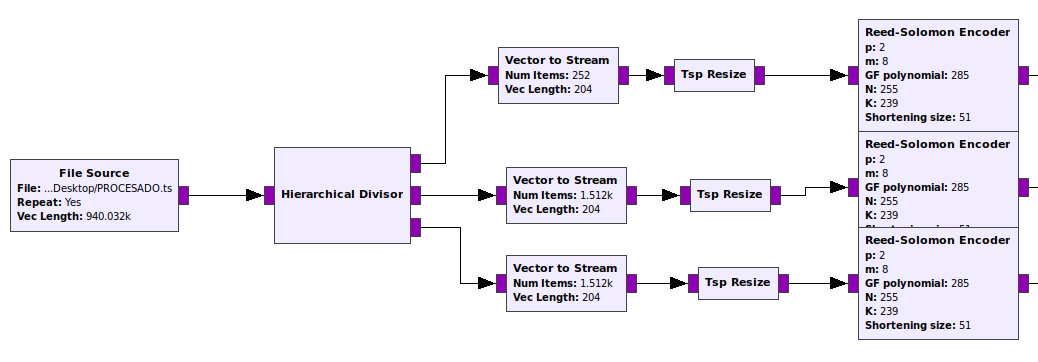
\includegraphics[scale=0.25]{h_div}
		\caption{Divisor jerárquico}
	\end{figure}
\end{frame}

%\subsection{El robustecimiento a nivel de datos}
\begin{frame}
\frametitle{El robustecimiento a nivel de datos}
\begin{itemize}	
	\item { Se aplican códigos correctores de errores a nivel de bits y bytes}
	\item {	Para aumentar la eficacia del código, se utilizan entrelazamientos}
	\item { Entrelazar implica agregar un retardo, que debe ser corregido }
\end{itemize}
\begin{figure}
	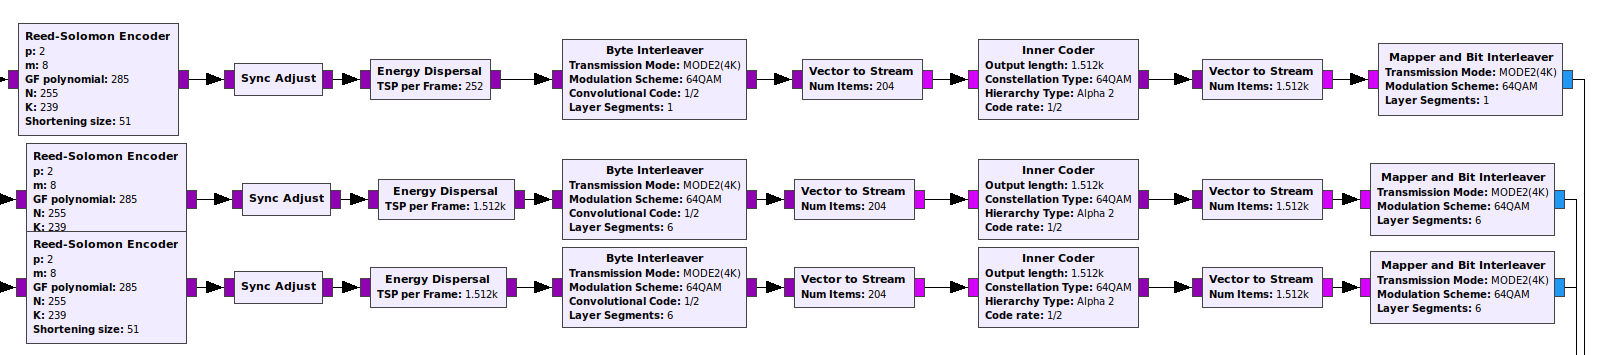
\includegraphics[scale=0.22]{rob_datos}
	\caption{Codificación de canal}
\end{figure}
\end{frame}
%\subsection{Mapeo y recombinación jerárquica}
\begin{frame}
\frametitle{Recombinacion jerárquica}
\begin{itemize}	
	\item { Se vuelven a entrelazar los datos, ahora mapeados en números complejos}
	\item {	Para aumentar la eficacia del código, se utilizan entrelazamientos}
	\item { Entrelazar implica agregar un retardo, que debe ser corregido }
\end{itemize}
\begin{figure}
	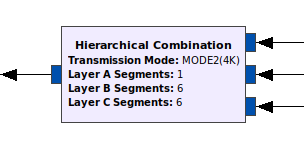
\includegraphics[scale=0.55]{h_conv}
	\caption{Combinador jerárquico}
\end{figure}
\end{frame}
%\subsection{El robustecimiento a nivel de portadoras}
\begin{frame}
\frametitle{El robustecimiento a nivel de portadoras}
\begin{itemize}	
	\item { Se realizan entrelazados en tiempo y frecuencia}
	\item {	El objetivo es mitigar los efectos del canal}
	\item { No es vital, pero mejora el desempeño en canales ruidosos }
\end{itemize}
\begin{figure}
	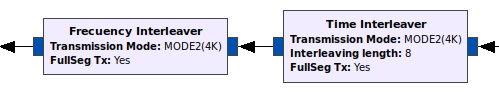
\includegraphics[scale=0.55]{rob_port}
	\caption{Bloques de entrelazamiento}
\end{figure}
\end{frame}
%\subsection{Formación del cuadro OFDM}
\begin{frame}
\frametitle{Formación del cuadro OFDM}
\begin{itemize}	
	\item { Se ubican los datos dentro de cada símbolo}
	\item {	Se agregan las portadoras piloto. Información de transmisión en las portadoras TMCC}
	\item { Agregamos portadoras dispersas para estimar el efecto del canal }
\end{itemize}
\begin{figure}
	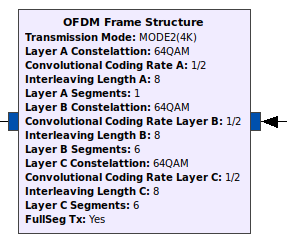
\includegraphics[scale=0.4]{bloque_ofdm}
	\caption{GNU Radio}
\end{figure}
\end{frame}

\begin{frame}
\frametitle{Formación del cuadro OFDM}
\begin{itemize}	
	\item { Ubicación de Portadoras de Datos y Portadoras Piloto}
	\item {	Agregamos información de transmision en las portadoras TMCC}
	\item { Agregamos portadoras dispersas para estimar el efecto del canal }
	\item { Agregamos portadoras auxiliares para enviar información extra (opcional) }
\end{itemize}
\begin{figure}
	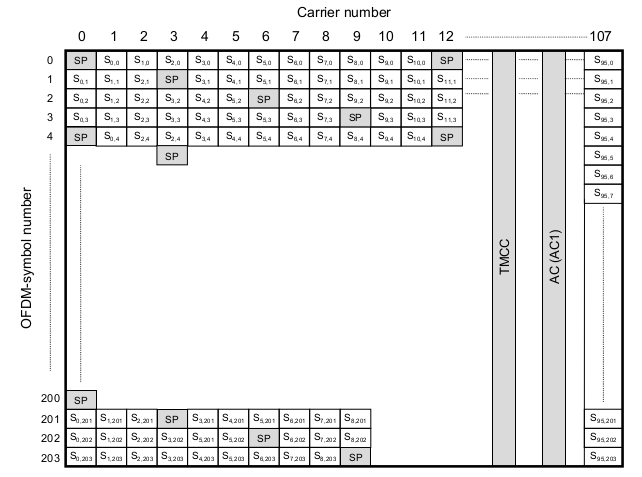
\includegraphics[scale=0.3]{ofdm_frame}
	%\caption{GNU Radio}
\end{figure}
\end{frame}
%\subsection{La puesta en el aire}
\begin{frame}
\frametitle{La puesta en el aire}
\begin{itemize}	
	\item { Mediante la transformada de Fourier pasamos al dominio del tiempo}
	\item {	Se agrega el prefijo cíclico}
	\item { Normalizamos los datos para la entrada al USRP }
	\item { Se determinan los parámetros de transmision en el equipo }
\end{itemize}
\begin{figure}
	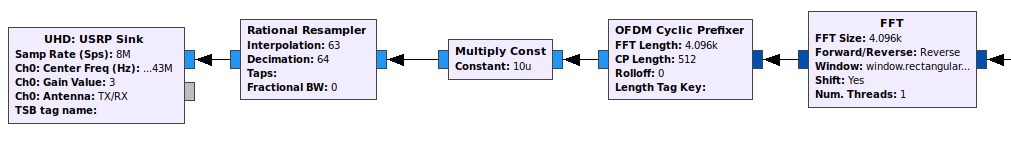
\includegraphics[scale=0.3]{final_tx}
	%\caption{GNU Radio}
\end{figure}
\end{frame}